\section{Genomförande} % (fold)
\label{sec:genomf_rande}
    \subsection{Steg 1} % (fold)
    \label{sub:steg_1}
        Projektet genomfördes med stöd av den valda metoden. I problemidentifikations-fasen, fas ett, hölls möten med uppdragsgivaren i syfte att få en enhällig uppfattning om vad företaget efterfrågade och formaliserade det praktiska problem som företaget sökte en lösning till. Vidare är det även i den här fasen som introduktionen till projektets rapport utvecklades för att fastslå vad projektet avser att utföra, som ett led i problemidentifieringen. \bigskip

        Den initiala problemanalysen resulterade i att projektet i stort kommer vara uppdelat i två mindre delar, dels den algoritm som klarar av att kalibrera panelen och dels en kommunikationslösning mellan panelen och rummet som den levererar ljuset till. \bigskip

        Förutsättningen vid litteraturstudien, gällande kommunikationen mellan taket och byggnadens innandöme, var att den trådlösa kommunikationen skall ske med standardiserade protokoll. Detta för att underlätta mottagandet av den trådlösa sändningen, i syfte att undvika tidssänken i felsökning då projektet har en relativt snäv tidsram.\bigskip

        För kalibreringsalgoritmens del, bestod problemförståelse steget av att undersöktes vilka typer av datastrukturer som skulle komma att beröras. När problemet analyserades insågs att värdena som samlas in kan representeras som en tvådimensionell matris (eng. 'array') där det finns ett unikt maxvärde och kring detta, minskande värden som blir lägre ju längre från maxvärdet de befinner sig, se figur\ref{fig:array}. \bigskip

        \begin{figure}[hbt]
        \centering
            \begin{subfigure}{0.2\textwidth}
                \pgfplotstabletypeset[color cells={min=5,max=9}, /pgfplots/colormap={yellowred}{rgb255(0cm)=(255,255,105); rgb255(1cm)=(255,10,10)},]
                {
                    5   6   7   6
                    6   7   8   7
                    7   8   9   8
                    6   7   8   7
                }
            \end{subfigure}
            \begin{subfigure}{0.2\textwidth}
                \pgfplotstabletypeset[color cells={min=3,max=9}, /pgfplots/colormap={yellowred}{rgb255(0cm)=(255,255,105); rgb255(1cm)=(255,10,10)},]
                {
                    6   7   8   9
                    5   6   7   8
                    4   5   6   7
                    3   4   5   6
                }
            \end{subfigure}
        \caption{\label{fig:array} Exempel på förväntade matriser}
        \end{figure}
    % subsection steg_1 (end)
    \subsection{Steg 2} % (fold)
    \label{sub:steg_2}
        Litteraturstudien resulterade i en förståelse att trådlösa standarder för datakommunikation så som 802.11 standarderna har problem att sända när betongkonstruktioner hindrar utspridningen av radiovågorna och kräver speciell apparatur för att klara av att skicka data igenom sådana förhållanden \cite{11n}. Detta medför att trådlös kommunikation inte är lämplig för företaget, då de på förhand inte kan veta ifall deras kommunikation kommer att fungera på plats hos deras kunder. \bigskip

        Ett lämpligare medium att kommunicera via är istället de fiberoptiska kablar som redan är dragna, då rummet lyses upp av just dessa kablar. Enligt företaget kommer det finnas mer än en fiberkabel dragen till varje rum, vilket öppnar upp för möjligheten att koppla in apparatur för kommunikation i en fiberkabel, medan den eller de andra kablarna kan fortsätta hämta in ljus till rummet. Med de svårigheter som den trådlösa kommunikationen medförde i kombination med att ett fungerande alternativt medium redan finns draget, valde projektet att fokusera på det senare. \bigskip

        Gällande kalibreringsalgoritmen framstod det vid datorkörningar att en algoritm som itererar över hela matrisen för att leta det högsta värdet kommer att vara väldigt ineffektiv. Ett beslut fattades att utveckla en algoritm som aktivt letar efter ett högre värde och som kräver så få steg som möjligt, detta då den praktiska implementationen kommer att innebära fördröjningssteg vid två punkter i körningen, dels när panelen flyttar på sig, och dels när ljuset ska hämtas in från lux-mätaren.

        \texttt{INSERT MORE TEXT ABOUT ALGORITHM HERE} \bigskip
    % subsection steg_2 (end)


    \subsection{Steg 3} % (fold)
    \label{sub:steg_3}
        Genom att fokusera på det optiska alternativet leder detta in projektet till det tredje steget i metoden, att föreslå en artefakt som löser det ställda problemet. Projektet föreslår då en lösning med en omvandlare från luxmätarens utdata till en optisk signal som sänds upp till taket för att där avkodas. Omvandlaren kan vara någon form av mikrokontroller så som till exempel en Arduino. Uppe på taken kan avkodaren även den vara en mikrokontroller, eller om det finns någon typ av ljussensor som direkt kan skicka sin data över USB till den programmerbara enhet som utför den algoritm som utvecklats. \bigskip

        Utformningen av algoritmen skedde genom flera iterationer av steg 3 i den valda metoden. I den första iterationen utvecklades en sökalgoritm, algoritm $\mathscr{A}$, som inledningsvis genomsöker en 3x3-matris i syfte att finna en inledande sökriktning. Därefter genomförs sökning medurs i åtta riktningar med utgångsriktning motsvarande österut. När ett större värde påträffas uppdateras nuvarande position och sökningen återupprepas. För jämförelse utvecklades även en variant med fyra sökriktningar, algoritm $\mathscr{B}$. Efterkommande iterationer var samtliga en vidareutveckling av den förra. Den andra iteration vidareutvecklade algoritmen så att den lagrar information om tidigare besökta koordinater, så att dessa ej undersöks vid upprepade tillfällen. Ytterligare förbättringar implementerades i den tredje iterationen, då riktningen på den senaste förflyttningen, då ett nytt större värde påträffats, registreras. Med hjälp av denna information undersöks först samma riktning som den senast lyckade förflyttningen innan medurs sökning. Här slopades också den inledande sökningen i 3x3 matris, då den inte kunde påvisas ha några märkbara fördelar. Samtliga iterationer innebar märkbara förbättringar vid simulering. Den slutgiltiga algoritmen arbetar enligt det flödesschema som finns presenterad i bilaga~\ref{sec:sokalgoritm_flow}. \bigskip

        \begin{figure}[hbt]
            \pgfplotsset{width=8cm,compat=1.8}
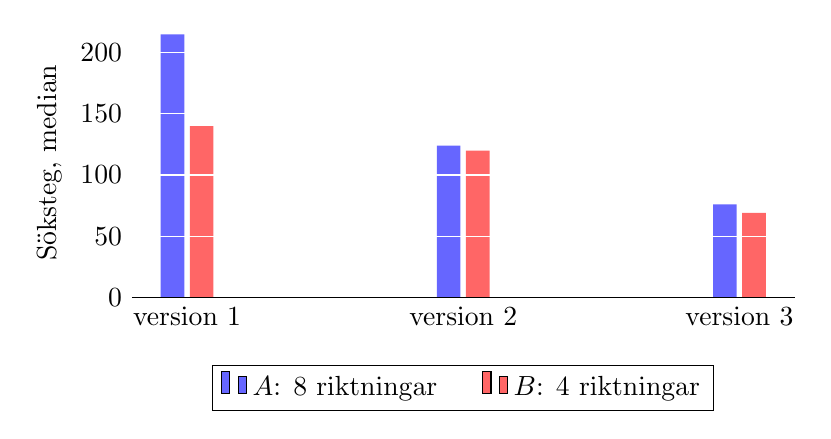
\begin{tikzpicture}
    \centering
    \begin{axis}[
        ybar,
        axis on top,
        % title={Söksteg algoritmer},
        height=5cm, width=10cm,
        bar width=0.3cm,
        ymajorgrids, tick align=inside,
        major grid style={draw=white},
        enlarge y limits={value=.1,upper},
        ymin=0, ymax=200,
        axis x line*=bottom,
        axis y line*=left,
        y axis line style={opacity=0},
        tickwidth=0pt,
        enlarge x limits=true,
        legend style={
            at={(0.5,-0.25)},
            % font=\footnotesize,
            anchor=north,
            legend columns=2,
            /tikz/every even column/.append style={column sep=0.5cm}
        },
        ylabel={Söksteg, median},
        symbolic x coords={version 1, version 2, version 3},
        xtick=data,
        % tick label style={font=\footnotesize},
        ]
        
        %% Median 8 riktningar
        \addplot [draw=none,fill=blue!60] coordinates {
            (version 1,215)
            (version 2,124) 
            (version 3,76)
        };

        %% Median 4 riktningar
        \addplot [draw=none, fill=red!60] coordinates {
            (version 1,140)
            (version 2,120) 
            (version 3,69)
        };
        \legend{$\mathscr{A}$: 8 riktningar,$\mathscr{B}$: 4 riktningar}
    \end{axis}
\end{tikzpicture}
        \caption{\label{fig:algoritm_steg} Jämförelse algoritmernas antal söksteg}
        \end{figure}

        För att jämföra sökalgoritmer genomfördes simuleringar för att mäta det antal steg som behövs för att ta sig från utgångspositionen till den position där det maximala värdet påträffades. Simuleringarna använde sig av 10000 100x100-matriser där varje matris hade slumpvist genererad utgångsposition och maximalt värde. Algoritmerna har alltså alla genomsökt samma matriser med samma utgångspositioner. Samtliga positioners värden var strängt avtagande i hänseende till avståndet från det maximala värdet. För varje iteration av algoritmen undersöktes sökning med både fyra och åtta sökriktningar. Sökning i fyra riktningar visade sig mer effektivt i samtliga fall, enligt figur~\ref{fig:algoritm_steg} och bilaga~\ref{sec:sokalgoritm_sim}. Skillnaderna i antal steg mellan samma algoritm med olika antal sökriktningar vara störst i den första iterationen, med 54~\% fler steg, men de visade sig även i övriga iterationer. I den tredje och slutgiltiga iterationen var skillnaden 10~\% fler steg. Varje iteration av algoritmen minskade det antal steg som behövdes för att finna det största värdet. Största förändringen mellan iterationer skedde mellan iteration två och tre, där antalet steg minskades med 43~\%, se tabell~\ref{tab:algoritm_forbattring}. Minskningen mellan iteration ett och tre var 51~\%. \bigskip

        \begin{table}[hb]
            \caption{\label{tab:algoritm_forbattring}Minskning av antal steg mellan varje version}
            \centering
            \begin{threeparttable}
            \begin{tabular}{@{}lcc@{}}
            \toprule
            Från        & \multicolumn{1}{l}{Till version 2} & \multicolumn{1}{l}{Till version 3} \\ \midrule
            Version 1 & 14~\%                                & 51~\%                                \\
            Version 2 & -                                    & 43~\% \\ \bottomrule
            \end{tabular}
            \begin{tablenotes}
            \item Baserat på medianvärden, se bilaga~\ref{sec:sokalgoritm_sim}
        \end{tablenotes}
        \end{threeparttable}
        \end{table}

    % subsection steg_3 (end)
% section genomf_rande (end)